\documentclass{standalone}
\usepackage{tikz}
\begin{document}
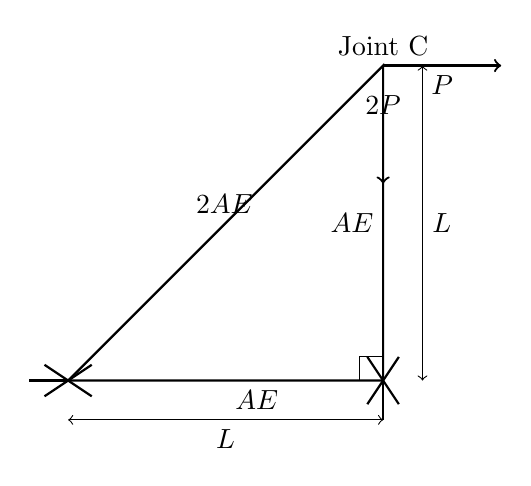
\begin{tikzpicture}
    % Coordinates
    \coordinate (A) at (0, 0);
    \coordinate (B) at (4, 0);
    \coordinate (C) at (4, 4);

    % Triangle
    \draw[thick] (A) -- (B) -- (C) -- cycle;

    % Supports
    \draw[thick] (A) -- ++(-0.5,0);
    \draw[thick] (A) ++(-0.3,0.2) -- ++(0.6,-0.4);
    \draw[thick] (A) ++(-0.3,-0.2) -- ++(0.6,0.4);
    \draw[thick] (B) -- ++(0, -0.5);
    \draw[thick] (B) ++(0.2,-0.3) -- ++(-0.4,0.6);
    \draw[thick] (B) ++(-0.2,-0.3) -- ++(0.4,0.6);

    % Load Arrows
    \draw[->, thick] (C) -- ++(0,-1.5 ) node[midway, above] {$2P$};
    \draw[->, thick] (C) -- ++(1.5,0) node[midway, below] {$P$};

    % Labels
    \node[above] at (C) {Joint C};
    \node[above right] at (1.5, 2) {$2AE$};
    \node[below right] at (2, 0) {$AE$};
    \node[left] at (4, 2) {$AE$};

    % Dimensions
    \draw[<->] (B) ++(0, -0.5) -- ++(-4, 0) node[midway, below] {$L$};
    \draw[<->] (C) ++(0.5, 0) -- ++(0, -4) node[midway, right] {$L$};

    % Right Angle
    \draw (B) ++(-0.3, 0) -- ++(0, 0.3) -- ++(0.3, 0);

\end{tikzpicture}
\end{document}
